\documentclass[tikz,border=10pt]{standalone}
\usepackage{pgfplots}
\usetikzlibrary{calc}

\begin{document}
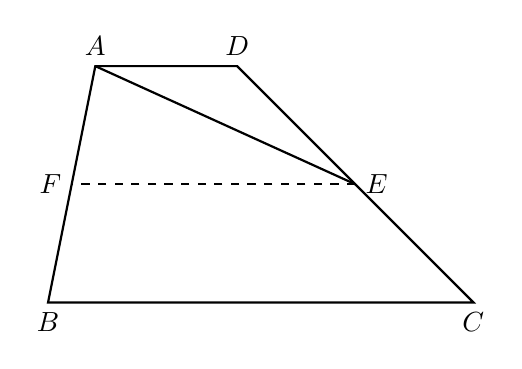
\begin{tikzpicture}[>=stealth, scale=1.2, thick]
    % --- 1. 定义关键顶点坐标 ---
    \coordinate (A) at (0.5, 2.5);
    \coordinate (D) at (2.0, 2.5);
    \coordinate (B) at (0, 0);
    \coordinate (C) at (4.5, 0);
    
    % --- 2. 定义点 E 和 F（核心新增：F 是 AB 中点）---
    \coordinate (E) at ($(D)!0.5!(C)$);
    \coordinate (F) at ($(A)!0.5!(B)$); % AB 中点 F 的计算

    % --- 3. 绘制图形边界 ---
    % 绘制梯形 ABCD
    \draw (A) -- (B) -- (C) -- (D) -- cycle;
    % 绘制连接线 AE
    \draw (A) -- (E);
    % 绘制虚线 EF（核心新增：黑色虚线）
    \draw[dashed] (E) -- (F);

    % --- 4. 标注顶点标签 ---
    \node[above] at (A) {$A$};
    \node[above] at (D) {$D$};
    \node[below] at (B) {$B$};
    \node[below] at (C) {$C$};
    \node[right] at (E) {$E$};
    \node[left] at (F) {$F$}; % 新增 F 点标签（左对齐，避免遮挡）

\end{tikzpicture}
\end{document}